\documentclass[12pt]{article}

\usepackage[utf8]{inputenc}
\usepackage[russian]{babel}
\usepackage{graphicx}
\usepackage{indentfirst}
\usepackage{booktabs}


\graphicspath{{pic/}}

\begin{document}

\begin{center}
	\LARGE 
	\textbf{Практическое занятие 6}\\
	АППРОКСИМАЦИЯ И ИНТЕРПОЛЯЦИЯ ДАННЫХ. МЕТОДЫ РЕШЕНИЯ ОБЫКНОВЕННЫХ ДИФФЕРЕНЦИАЛЬНЫХ УРАВНЕНИЙ\\
\end{center}

\begin{flushright}
	\large
	Игнашов Иван\\
	Вариант 8\\
\end{flushright}

\newpage

 \section*{1. Цель работы}
Изучение основных методов аппроксимации и интерполяции данных в системе MATLAB и способов решения ОДУ
\subsection*{Порядок работы:}
\begin{enumerate}
	\item С помощью интерполяции найти значение таблично заданной функции в указанной точке\\
		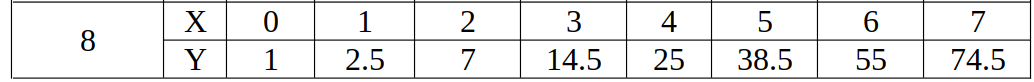
\includegraphics[width=0.75\linewidth]{formula.png}\\
		
	\item Выполнить аппроксимацию той же таблично заданной функции\\
	
	\item Найти определенный интеграл для той же подынтегральной функции с использованием пакета символьных вычислений\\
\end{enumerate}

\newpage
 \section*{2. Листинг программы}%
 
 \subsection*{2.1. графики f1, f2, f3}
\begin{figure}[!h]
	\centering
	%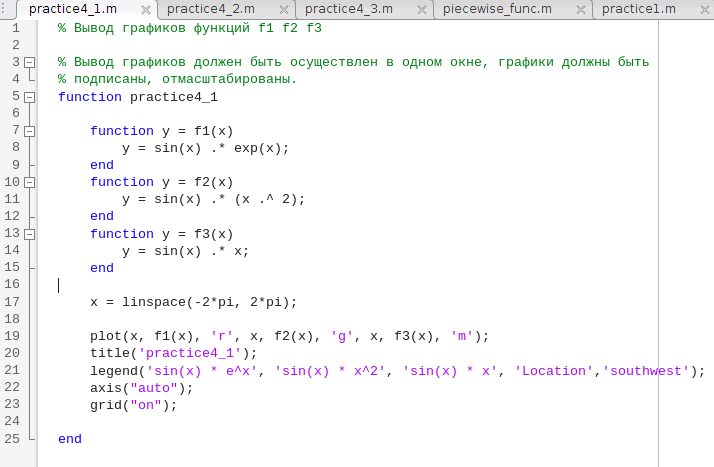
\includegraphics[width=\linewidth]{multiple_lines.png}
	\caption{Программа генерации графиков f1, f2, f3}
\end{figure}

\begin{figure}[!h]
  \subsection*{2.2. трёхмерная поверхность f4}
 \end{figure}
 
 
\begin{figure}[!h]
 \subsection*{2.3. график кусочно-заданной функции} 
\end{figure}

\section*{3. Результаты выполнения}
 

\end{document}